\chapter{Evaluación experimental}
\label{chap:evaluacion_experimenal}
Para comprobar que os resultados obtidos correspóndense co plantexado probaremos o dispositivo e a aplicación. Realizaremos probas en contornos controlados e probas no medio real o que esta dirixido.

\section{Consumo e autonomía}

Comenzarase as probas medindo o consumo de amperios do sistema. Para elo colocarase un amperímetro usb entre unha fonte de alimentación e a conexión usb coa que alimentarase o sistema nestas probas. Repetiremos as probas con diferentes fontes de alimentación e distintos cables para descartar fallos e conseguir unha maior consistencia nos resultados. A continuación realizaranse as mesmas probas no dispositivo medindo o consumo alimentándoo coa batería.

Analizaranse os seguintes supostos para o dispositivo con un anel led e para o que conta a maiores coas dúas tiras led.
\begin{itemize}
    \item \textbf{Sistema en repouso: }
    O sistema esta aceso pero só se estean a executar as funcións do sistema operativo incluíndo o servidor ssh para o control remoto.
    \item \textbf{Servidor funcionando:}
    Executamos o servidor.
    \item \textbf{Cliente conectado:}
    Conectamos o dispositivo móbil o servidor.
    \item \textbf{Vídeo transmitindo:}
    Transmitimos vídeo en directo o dispositivo móbil.
    \item \textbf{Vídeo parado:}
    Paramos a transmisión de vídeo.
    \item \textbf{Desconexión do cliente:}
    Pechamos a aplicación no dispositivo móbil.
    \item \textbf{Luces intermitentes:}
    Iniciamos as luces intermitentes a máxima intensidade nunha das direccións, consumo varia no proceso, rexistremos o valor máximo.
    \item \textbf{Luces vermellas:}
    Acendemos as luces vermellas a intensidade máxima.
    \item \textbf{Luces vermellas e transmisión de vídeo:}
    Consumo coas luces vermellas a máxima intensidade e co vídeo transmitindo en directo.
\end{itemize}

\begin{figure}[tb]
  \centering
  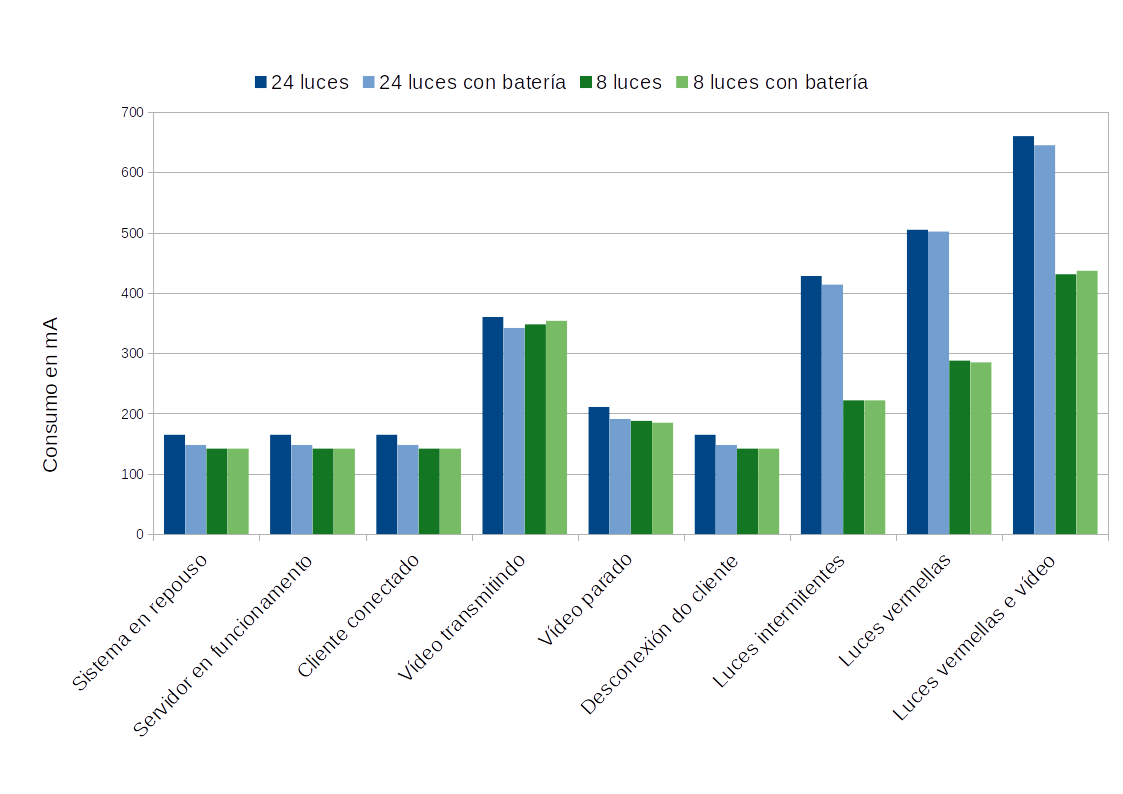
\includegraphics[scale=.5]{imaxes/grafica-amperaxe.png}
  \caption{Grafica do consumo en mA.}
  \label{f:soporte móbil}
\end{figure}
Como se pode observar na gráfica da figura 5.1 o uso ou non de batería non afecta en gran medida ao consumo de amperios, pero ha de terse en conta que estas probas realizáronse coas batería coa carga completa. Se comparamos a previsión de consumos que fixemos coas medición obtidas 

As fontes de alimentación utilizadas poden proporcionar un máximo de 3A e 2.1A respectivamente, tamén utilizáronse dous cables un de maior calidade e outro cunha calidade inferior. En ningún dos casos obtivéronse diferencias apreciables sendo a maior diferencia de 4mA. Na versión con batería necesitouse utilizar cableado a maiores para realizar as probas, o que pode que incrementara lixeiramente o consumo.

A seguinte proba a realizar será a de autonomía do dispositivo, para elo buscarase o consumo máximo acendendo as luces vermella a máxima intensidade o tempo que se transmite vídeo.

Comezaranse as probas co dispositivo dotado de batería interna, cando a voltaxe da batería esta entorno os 3.7V detectase un problema o sistema apagase, indicando batería baixa. O \emph{script} Python encargado de monitorizar o pin conectado o indicador de voltaxe baixo do Adafruit Powerboost detecta unha caída de voltaxe que confunde co franco de caída esperado cando o pin ponse a 0. O pin de baixo voltaxe do Adafruit Powerboost está conectado a voltaxe da batería cando a caga e superior a 3.2V e conectase a un valor de 0V cando baixa de este limite e debido a que cando batería esta a comezar a descargarse para poder proporcionar a amperaxe adecuada a súa voltaxe baixa a un ritmo rápido que confunde o \emph{script}. O podemos solucionar incluíndo unha segunda comprobación no \emph{script} despois de detectar o franco de caída comprobarase que o valor lido no pin é 0 antes de apagar a Raspberry.

A continuación detectase un segundo problema, despois de  min volvese a apagar por batería baixa e unha vez apagado a batería recuperase ata unha voltaxe de 3.5V. Esto debese a que o estar consumindo o máximo de amperios necesita baixar a súa voltaxe para poder seguir entregando estes amperios. Que o sistema se apague neste punto e conveniente para protexer a batería e prolongar a súa vida útil pero reduce o tempo de uso da batería, que poderíamos seguir usando sempre que non utilicemos o consumo máximo do dispositivo. Este problema pódese solucionar de dúas formas:
Utilizando un batería de maior capacidade xa que poderá seguir subministrando a amperaxe necesaria a menor voltaxe.
Utilizar unha batería cunha constante de descarga maior, isto é a capacidade máxima de amperios que pode subministrar en función da capacidade en amperios hora. A batería utilizada ten unha constante de descarga de 1C isto quere dicir que coa sua caga completa o fabricante garante que proporcione 1.6A funcionando con normalidade.
Ámbalas dúas solucións implican na practica unha batería de maior tamaño.

Procedemos a repetir a proba pero esta vez deshabitando o apagado automático, esperando a que o sistema se apague cando a voltaxe non sexa suficiente para manter a Raspberry acesa ou no peor caso cando o circuíto de protección que inclúe a batería a desconecte a 2.5V. De non usar unha batería con circuíto de protección poderíamos danar a batería podendo incluso arder ou estoupar durante próximas cargas. Neste caso obtemos minutos de funcionamento.

Comezarase as probas para a versión do dispositivo sen luces intermitentes, faremos a proba cunha batería de 6000mA, obtense    , Neste caso observase que cando o dispositivo non pode subministrar suficiente voltaxe para alimentar a Raspberry esta se apaga, e como consecuencia tamén os leds alimentados dende o seu \emph{power rail}, o diminuír o consumo a voltaxe volve a ser suficiente para alimentar a Rasberry polo que esta se reinicia, entrando desta forma nun ciclo de reinicios ata que a voltaxe non e suficiente para arrancar a Raspberry.

\section{Vídeo e lentes}
Nesta sección procederase a analizar a calidade do vídeo obtida a latencia
\section{Visibilidade}

\section{Estabilidade e consumo da aplicación}
